\documentclass[../main/main.tex]{subfiles}
\begin{document}

\dominitoc
\faketableofcontents
\dominilof
\fakelistoffigures
\dominilot
\fakelistoftables

\chapter{Impact sur la cosmologie~: simulations}\label{ch:sims}
\epigraph{\openquote\textit{The Answer to the Great Question… Of Life, the
    Universe and Everything… Is… Forty-two.}\closequote}{Douglas \textsc{Adams},
    \textit{H2G2}}

Nous avons vu dans le chapitre précédent la manière dont \snana\ permettait de
traiter les biais et corrélations environnementales dans le calcul des
paramètres cosmologiques, et ainsi pourquoi son utilisation dans notre thèse
était pertinente.

Dans ce chapitre, nous présentons les simulations que nous avons effectuées avec
le logiciel. Dans un premier lieu, nous discutons des différentes corrélations
que nous avons testées \textit{via} l'utilisation de \hostlib\
(Section~\ref{sec:hpres}) et de la confection de nôtres
(Section~\ref{sec:hmake}). Par la suite, nous introduisons…

\vfill
\minitoc
\vfill

\newpage

\section{Présentation des \hostlib}\label{sec:hpres}

Dans sa forme la plus générale, une \hostlib\ ne possède pas de valeurs liées à
des paramètres de SNe~Ia (comme l'étirement ou la couleur)~; en effet, elle sert
originellement à utiliser le redshift photométrique de la galaxie hôte comme
valeur antérieure dans l'ajustement du redshift de la SN et à ajouter du bruit à
la SN simulée (voir Chapitre~\ref{ch:snana}). Avant d'intégrer notre modèle à
\snana, il nous a fallu reproduire les approches d'autres groupes utilisant le
logiciel. Nous avons choisi pour cela les études de~\cite{scolnic2016}, ci-après
SK\defcitealias{scolnic2016}{SK}, et de~\cite{popovic2021a}, ci-après
BP\defcitealias{popovic2021a}{BP}.

% However, the definition of a realistic model is the be questioned. In the
% pioneer work of \cite{scolnic2016}, there were no relationship between SNe and
% their host galaxy. \cite{popovic2021a} and~\cite{smith2020} introduced a link
% between the two thanks to a HOSTLIB: a table of 100,000 galaxies made to mimic
% the actual surveyed galaxies by the different samples. To each galaxy is
% associated a SN through its main fitted properties such as $x_1$ or $c$, which
% are generated by models of underlying distributions. Yet, this process was
% directed at guessing what relationship would fit more the data, by using bins of
% host galaxy masses and minimizing asymmetric Gaussian distributions for each in
% a backward-modeling way. It's a non-direct method to infer an evolution of an
% underlying distribution as a function of mass.
% 
% Our approach was to use independent data from the SNf sample that uses LsSFR to
% characterize a galaxy, as explained in Section~\ref{sec:model}, and make an
% evolving, analytical model that can then describe higher-redshift SNe in a
% forward-modeling approach. This method has the aim to be predictive and to
% better fit the data, as is discussed in Section~\ref{sec:results}. In order to
% implement our modeling in this framework, we had to modify the HOSTLIBs on which
% the simulations are based.

% SK16 is galaxy distribution from which you draw, P21 is a list with the
% distrubtion already in it, linking the relationships and $x_1$ and stuff
% already drawn. But there's no evolution in it, and we want to do that. Forward
% model that through.

% General, Brodie, us; no lightcurve fitting, and at the end of hostlib section
% w simulate antheon

% P21: There is a relationship, we'll try to guess it. Take data bns of mass,
% and calculate what the distribtion of stretch is for each. Looks differently
% in different bins: as a function of mass they have distribution. Backward
% models.  N21: our data is independent and we use it to show that it works on
% other data at higher redshift, is predictive, and involves an evolution of the
% distributions.

% Generate $z$, take closest $M$ entry in a table of host galaxies (HOSTLIB),
% then pick $x_1$, $c$ assuming underlying relationships defined by the BBC
% team.  Because we want to make these simulations with an evolving underlying
% distribution, we have to replace then $x_1$ values by what is estimated by our
% previous model.

\subsection{Étirement et couleur globales~: SK}\label{ssec:sk}

Dans leurs travaux, \citetalias{scolnic2016} n'incluent pas de lien d'étirement
ou de couleur avec les propriétés de la galaxie hôte mais uniquement une marche
de magnitude en fonction de sa masse $M_*$. Celle-ci est inclut dans les
\wgtmap\ des sondages, et est de \SI{0.05}{mag}. Le tirage des paramètres $x_1$
et $c$ se font alors depuis des distributions asymétriques Gaussiennes, décrites
par~:
\begin{equation}\label{eq:skasym}
    P(p) = \left\{
        \begin{array}{l}
            e^{-\DS\frac{\abs{p-\mu}^2}{\sigma_-{}^2}
                \quad\text{si}\quad p\leq\mu} \\
            e^{-\DS\frac{\abs{p-\mu}^2}{\sigma_+{}^2}
                \quad\text{si}\quad p>\mu} \\
        \end{array}
        \right.
\end{equation}
avec $p = x_1$ ou $c$. Les valeurs des paramètres sont indiqués
Tableau~\ref{tab:skasym}.

\begin{table}[h]
    \centering
    \begin{threeparttable}
        \caption[Paramètres des distributions d'étirement et de couleur pour les
        simulations SK]{Paramètres des distributions sous-jacentes d'étirement
            et de couleur desquelles sont générées les SNe~Ia dans notre
        reproduction du travail de \citetalias{scolnic2016}.}
        \label{tab:skasym}
        \begin{tabular}{lcccccc}
            \toprule
            \multirow{2}[2]{*}{Sondage} &
            \multicolumn{3}{c}{$x_1$} &
            \multicolumn{3}{c}{$c$}\\
            \cmidrule(lr){2-4} \cmidrule(lr){5-7} &
            $\mu$ & $\sigma_-$ & $\sigma_+$ &
            $\mu$ & $\sigma_-$ & $\sigma_+$ \\
            \midrule
            PS1    &
            0,604  & 1,029 & 0,363   &
            -0,077 & 0,029 & 0,12\\
            SDSS   &
            1,141  & 1,653 & 0,100   &
            -0,038 & 0,048 & 0,079\\
            SNLS   &
            0,964  & 1,232 & 0,282   &
            -0,065 & 0,044 & 0,12\\
            LOWZ   &
            --     & --    & --      &
            -0,055 & 0,023 & 0,015\\
            \bottomrule
        \end{tabular}
        \begin{tablenotes}[flushleft]
        \item\small \textbf{\hspace{-3,2pt}Notes.} Les valeurs viennent du
            Tableau~1 de \citetalias{scolnic2016}, sauf pour LOWZ dont la
            distribution d'étirement est une double Gaussienne
            d'après~\cite{scolnic2018}.
        \end{tablenotes}
    \end{threeparttable}
\end{table}

Nous avons cependant utilisé les valeurs de paramètres de~\cite{scolnic2018}
pour la distribution d'étirement de LOWZ, qui est alors décrite par une
combinaison de deux Gaussiennes dont une asymétrique, telle que~:
\begin{equation}\label{eq:sklowz}
    P(x_1) = A_1\times
        \left\{
        \begin{array}{l}
            e^{-\DS\frac{\abs{x_1-\mu_1}^2}{\sigma_{-,1}{}^2}
                \quad\text{si}\quad x_1\leq\mu_1} \\
            e^{-\DS\frac{\abs{x_1-\mu_1}^2}{\sigma_{+,1}{}^2}
                \quad\text{si}\quad x_1>\mu_1} \\
        \end{array}
        \right. + A_2\times
        e^{-\DS\frac{\abs{x_1-\mu_2}^2}{\sigma_{2}{}^2}}
\end{equation}
Les valeurs sont indiquées Tableau~\ref{tab:sklowz} avec le rapport d'amplitude
$a=\frac{A_1}{A_2}$. 

\begin{table}[ht]
    \centering
    \begin{threeparttable}
        \caption[Paramètres de la distribution d'étirement pour l'échantillon
        LOWZ des simulations SK]{Paramètres de la distribution sous-jacente
            d'étirement pour l'échantillon LOWZ dans notre reproduction de
        l'étude de~\citetalias{scolnic2016}.}
        \label{tab:sklowz}
        \begin{tabular}{lcccccc}
            \toprule
            \multirow{2}[2]{*}{Sondage} &
            \multicolumn{6}{c}{$x_1$}\\
            \cmidrule(lr){2-7} &
            $\mu_1$ & $\sigma_{-,1}$ & $\sigma_{+,1}$ &
            $a$ &
            $\mu_2$ & $\sigma_{2}$ \\
            \midrule
            LOWZ &
            0,55 & 1,0 & 0,45  &
            0,55 &
            -1,5 & 0,5 \\
            \bottomrule
        \end{tabular}
        \begin{tablenotes}[flushleft]
        \item\small \textbf{\hspace{-3,2pt}Notes.} Les caractéristiques sont
            celles reportées dans l'annexe C de~\cite{scolnic2018}, mais les
            valeurs y étant erronées nous avons utilisé celles de l'équipe
            directement.
        \end{tablenotes}
    \end{threeparttable}
\end{table}

\subsection{Étirement et couleur selon la masse~: BP}\label{ssec:bp}

D'un autre côté, \citetalias{popovic2021a} définissent des distributions mères
Gaussiennes asymétriques pour $x_1$ et $c$ selon la masse de la galaxie hôte.
Ceci est effectué en découpant les données des sondages en intervalles selon
$M_*$~; dans chacun de ces intervalles sont déterminés les paramètres des
Gaussiennes asymétriques, puis à chaque entrée de la \hostlib\ sont sélectionnés
des paramètres d'étirement et de couleur selon la valeur de la masse de la
galaxie hôte. Ainsi, par rapport à SK, ces \hostlib\ présentent 2 colonnes
supplémentaires, une pour $x_1$ et une pour $c$, attribuant à chaque entrée une
valeur de ces paramètres à associer à la SN simulée. 

Ce procédé est réalisé pour LOWZ d'une part, menant à une \hostlib\ que nous
appelons «~BP\_lowz~», et pour la combinaison des sondages DES, SDSS, PS1 et
SNLS d'autre part, menant à une \hostlib\ que nous nommons «~BP\_highz~». Les
valeurs des paramètres correspondants sont disponibles dans l'annexe A2
de~\citetalias{popovic2021a}.

Ce sont ces \hostlib\ qui constituent la base de notre étude~; en réalité, les
\hostlib\ SK sont celles de BP où nous avons retiré le tirage des colonnes $x_1$
et $c$.

\subsection{Étirement selon l'âge~: NN}\label{ssec:nn}

Pour notre étude, nous avons besoin de relier l'étirement attribué à la SN avec
l'âge de son environnement, en correspondance avec nos travaux précédents
\citep[][ci-après NN]{nicolas2021}\defcitealias{nicolas2021}{NN}. Nous avons
alors pris les \hostlib\ BP pour y remplacer la colonne d'étirement par les
valeurs attendues de notre modèle et y ajouter une colonne \texttt{LOGsSFR}
indiquant si la SN est jeune (\texttt{LOGsSFR}=1) ou vieille
(\texttt{LOGsSFR}=0), et nommons ces \hostlib\ «~NN~». La réalisation de cette
\hostlib\ est présentée dans la Section~\ref{sec:hmake}.

\subsection{Étirement et marche de magnitude selon l'âge~: NR}\label{ssec:nr}

Comme nous l'avons vu précédemment, l'âge des SNe~Ia a une double implication~:
celle de l'évolution de la distribution sous-jacente de l'étirement avec le
redshift (Chapitre~\ref{ch:stretch}), mais aussi une marche de magnitude de
$\gamma_{\rm env} = \SI{0,13}{mag}$ entre les SNe~Ia jeunes et vieilles
\citep[Chapitre~\ref{ch:stretch},][]{rigault2020}. Nous avons implémenté cette
valeur à la place de la marche de magnitude selon $M_*$ incluse dans les
\wgtmap\ des sondages \textit{via} l'ajout d'une colonne \texttt{SNMAGSHIFT} aux
\hostlib\ NN~: ces nouvelles \hostlib\ se nomment «~NR~» pour «~\textsc{Nicolas}
\textsc{Rigault}~», et présentent l'exacte même colonne d'étirement que les NN.

\section{Confection des \hostlib}\label{sec:hmake}

Afin de simuler des SNe~Ia avec notre modèle, que ce soit pour NN ou NR, nous
avons besoin que les propriétés des galaxies hôtes suivent les distributions de
ce qui a été observé par les différents sondages simulés. Bien que nous
soutenions que le LsSFR est un meilleur traceur de l'environnement d'une SN
\citep{briday2022}, la plupart des sondages caractérisent les galaxies avec leur
masse stellaire. Ainsi, la colonne des $M_*$ des \hostlib\
\citetalias{popovic2021a} reste intacte puisque leurs couleurs (que nous
utilisons) utilisent les intervalles de $M_*$.

Étant donné que le LsSFR repose sur la masse de la galaxie hôte\footnote{pour
rappel~: $\mathrm{sSFR} = \frac{\rm SFR}{M_*}$}, nous ne pouvons pas uniquement
nous baser sur la valeur du redshift $z$ d'une entrée des \hostlib\ BP pour y
assigner un étirement. Nous attendons effectivement que les galaxies vers
$M_*\approx12$ ne contiennent des SNe~Ia vieilles (c'est-à-dire LsSFR $\approx$
0) alors que les galaxies de $M \gtrsim 7$ n'en contiennent que des jeunes
(LsSFR $\approx$ 1).

Par conséquent, afin de comparer les implications de notre modélisation basée
sur le LsSFR avec ce que les autres sondages ont observé, nous avons dû
modéliser les masses des galaxies hôtes par rapport au LsSFR~; nous avons pour
cela utilisé le même échantillon du Chapitre~\ref{ch:sample} que pour la
modélisation de l'étirement du Chapitre~\ref{ch:stretch}. Cependant, nous
soulignons que cette étude n'a pas pour volonté de décrire l'évolution des
masses des galaxies hôtes (qui sont des propriétés globales) avec le LsSFR d'une
supernova (étant une propriété intrinsèque de celles-ci)~: son utilité est
d'associer de manière cohérente un âge à une SN caractérisée par un certain
redshift et par une masse de galaxie hôte.

\subsection{Modélisation du lien entre masse et redshift}\label{ssec:mmod}

De la même manière que dans le Chapitre~\ref{ch:stretch}, nous utilisons le
LsSFR comme traceur de l'âge d'une SN, mais cette fois sur les estimations de
masse du sondage SNf. Ensuite nous modélisons les populations jeune et vieille
par une série de paramétrisations différentes et choisissons celle qui a le plus
faible AIC. Cependant, les masses SNf ont été calculées à l'aide de l'Équation~8
de~\cite{taylor2011} (voir~\cite{rigault2020}) alors que d'autres études du
catalogue Pantheon utilisent différentes techniques d'estimation de la masse qui
pourraient donner des valeurs de sortie différentes pour une même galaxie.

L'estimation de \textsc{Taylor} utilise la magnitude AB absolue en bande $i$
d'une galaxie, $M_i$. Elle est déduite de la magnitude apparente $m_i$
connaissant le redshift de la galaxie mais suppose que la bande $i$ observée est
proche de celle du référentiel de repos, ce qui est vrai pour les redshift de
SNf qui sont inférieurs à $z\approx 0,05$. Les relevés de l'échantillon Pantheon
sont à des redshifts plus élevés et ont utilisé un ajustement des distributions
spectrales d'énergie (en anglais SED pour \textit{spectral energy
distributions}) des galaxies pour éviter les corrections K dans cette procédure.

Nous avons appliqué la même analyse à l'échantillon SNf~; les données ainsi
calculées sont nommées «~SEDSNf~» par la suite, et l'échantillon fiduciel
utilisant SEDSNf est nommé «~SED fiduciel~». À cause de l'absence de 4 galaxies
hôtes dans les catalogues de données nécessaire à ce calcul, l'échantillon
SEDSNF est réduit à 110 données, au lien de 114 pour SNf. Nous indiquons
également que nous nous limitons pour cette étude aux galaxies de $M_* >
10^7\si{\Msun}$, étant donné que les valeurs inférieures servent à indiquer
qu'aucune galaxie hôte n'a été définie~; le sondage fiduciel tombe alors à 548
données, et SED Fiduciel à 544.

Nous avons donc réalisé cette étude de l'évolution des distributions
sous-jacentes de masse avec le LsSFR en utilisant~:
\begin{enumerate}
    \item [\bfseries SNf] Uniquement les données de SNf (masses issues d'un
        calcul par l'Équation de \textsc{Taylor})~;
    \item [\bfseries SEDSNf] Uniquement les données de SNf avec les masses
        issues d'un ajustement par SED~;
    \item [\bfseries Fiduciel] Toutes les données de notre échantillon
        fiduciel~;
    \item [\bfseries SED fiduciel] Toutes les données de notre échantillon
        fiduciel avec les masses SEDSNF.
\end{enumerate}

\begin{figure}[t]
    \centering
    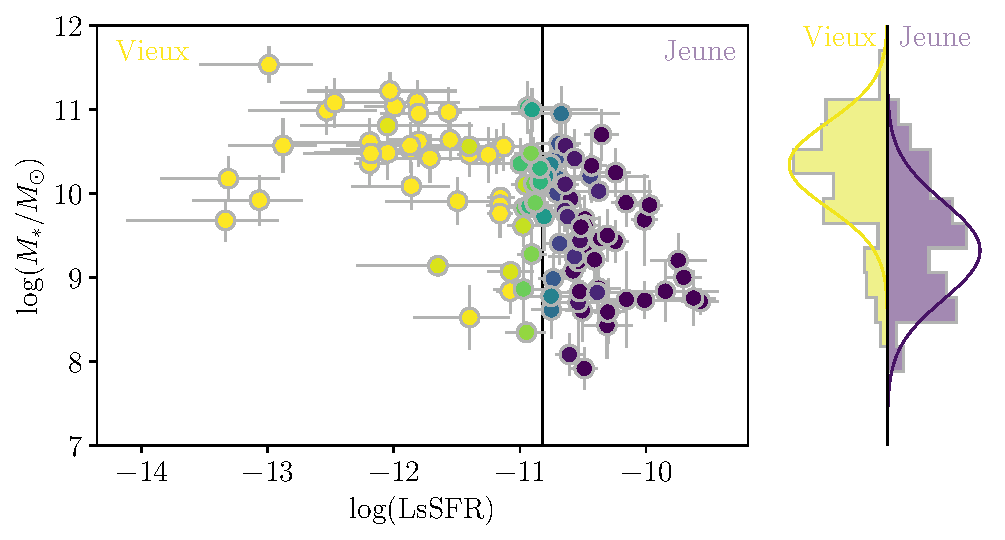
\includegraphics[width=\linewidth]{model_mass_Howell_hist_SED-nonan.pdf}
    \caption[$M_*$ en fonction du LsSFR des SNe~Ia de SNfactory et modèle de
    masse sélectionné ajusté]{\textit{Principal}~: masses des galaxies hôtes
        ($M_*$) ajustées par SED en fonction du LsSFR pour les SNe de SNfactory.
        La couleur correspond à la probabilité $p_y$ que la SN~Ia soit jeune,
        c'est-à-dire qu'elle ait $\log \mathrm{LsSFR} \geq -10,82$
        \citep[voir][et Chapitre~\ref{ch:stretch}]{rigault2020}. \textit{À
        droite}~: histogramme pondéré par $p_y$ des étirements des SNe, ainsi
        que le modèle sélectionné ajusté~; les contributions des populations
    jeune et âgée sont indiquées en violet et jaune, respectivement.}
    \label{fig:massmodel}
\end{figure}

D'après la forme des histogrammes de la Figure~\ref{fig:massmodel}, nous avons
implémentés différentes modélisations. Cette étude étant annexe à la simulation
par \snana, nous ne présentons que les plus pertinentes et omettons les
modélisations n'ayant pas d'intérêt physique ou mathématique, c'est-à-dire les
modélisations constantes avec le redshift (notamment les Gaussienne simple et
Gaussienne asymétrique pure) et les modèles ne convergeant pas. Ainsi, nous
présentons les modèles suivants~:

\begin{itemize}
    \item «~Howell~» d'après~\cite{howell2007}, avec une Gaussienne simple pour
        chacune des populations jeune et âgée (voir Chapitre~\ref{ch:stretch})~;

    \item «~Howell+asym~» où la population jeune est une simple Gaussienne et la
        population vieille est une Gaussienne asymétrique~;

    \item «~Howell asym~» où les deux populations jeune et âgée sont
        asymétriques.
\end{itemize}

\subsection{Comparaison aux données}\label{ssec:mres}

Chacun de ces modèles a été ajusté aux différents échantillons, et nous en
présentons maintenant les résultats. La procédure d'ajustement est celle de la
Section 3 de~\citetalias{nicolas2021}, selon la présence de LsSFR dans chaque
sous-échantillon. On définit de même que précédemment
\begin{equation}\label{eq:likelihood}
    -2\ln(L) = -2 \sum_i \ln \prob{x_1^i}{\vec{\theta};
    \mathrm{d}x_1^i, y^i}.
\end{equation}
et nous utilisons le critère d'information
d'\textsc{Akaike}~\citep[AIC,][]{burnham2004} pour comparer la capacité de
chaque modèle à décrire correctement les données en pénalisant l'ajout de
paramètres libres tel que~:
\begin{equation}
    \mathrm{AIC} = -2\ln(L) + 2k,
\end{equation}
ce qui permet d'éviter le sur-ajustement. Les résultats sont présentés
Tableau~\ref{tab:modelcomp}.

\begin{table}[h]
    \centerfloat
    \begin{threeparttable}
        \caption[Comparaison de la capacité relative de chaque modèle à décrire
        les données selon l'échantillon d'ajustement]{Comparaison de la
            capacité relative de chaque modèle à décrire les données selon
        l'échantillon d'ajustement.}
        \label{tab:modelcomp}
        \begin{tabular}{lcccccccccc}
            %\hline\hline & & & & & & \\[-0.6em]
            \toprule &
            & \multicolumn{3}{c}{Howell ($k=4$)}
            & \multicolumn{3}{c}{Howell+asym ($k=5$)}
            & \multicolumn{3}{c}{Howell asym ($k=6$)} \\
            \cmidrule(lr){3-5}\cmidrule(lr){6-8}\cmidrule(lr){9-11}
            Échantillon & N$_{\rm SNe~Ia}$ &
            $-2\ln(L)$ & AIC & $\Delta$AIC &
            $-2\ln(L)$ & AIC & $\Delta$AIC &
            $-2\ln(L)$ & AIC & $\Delta$AIC\\[0.2em]
            %\hline & & & & & & \\[-0.6em]
            \midrule
            SNf & 114 &
            230,0 & 238,0 & -- &
            229,8 & 239,8 & -1,8 &
            229,7 & 241,7 & -3,7 \\
            SEDSNf & 110 &
            223,9 & 231,9 & -- &
            221,4 & 231,4 & 0,6 &
            221,3 & 233,3 & -1,4 \\
            Fiduciel & 544 &
            1534,3 & 1542,3 & -- &
            1534,3 & 1544,3 & -2,0 &
            1531,0 & 1543,0 & -0,7 \\
            SED Fiduciel & 548 &
            1546,6 & 1554,6 & -- &
            1546,5 & 1556,5 & -1,9 &
            1538,7 & 1550,7 & 4,0 \\
            \bottomrule
        \end{tabular}
        \begin{tablenotes}[flushleft]
            \item\small \textbf{\hspace{-3.2pt}Notes.} Pour chaque modèle
                considéré, nous indiquons son nombre
                de paramètres libres $k$, et pour chaque échantillon étudié son
                $-2\ln(L)$ (voir Équation~\ref{eq:likelihood}), son AIC et la
                différence d'AIC ($\Delta$AIC) entre ce modèle et le modèle
                Howell, choisi comme référence car présentant l'AIC le plus
                faible pour 6 comparaisons sur 8.
        \end{tablenotes}
    \end{threeparttable}
\end{table}

Après calcul, le modèle Howell est celui qui se détache le plus, étant celui de
plus petit AIC pour 6 modèles sur 8, et est celui représenté sur la
Figure~\ref{fig:massmodel}~; cependant tous les modèles sont considérés comme
étant de bonnes représentations des données. Nous présentons
Figure~\ref{fig:mod_comp} une illustration des résultats du tableau précédent,
et Figure~\ref{fig:mod_all} les représentations graphiques des modèles
implémentés variant en redshift.

\begin{figure}[ht]
    \centering
    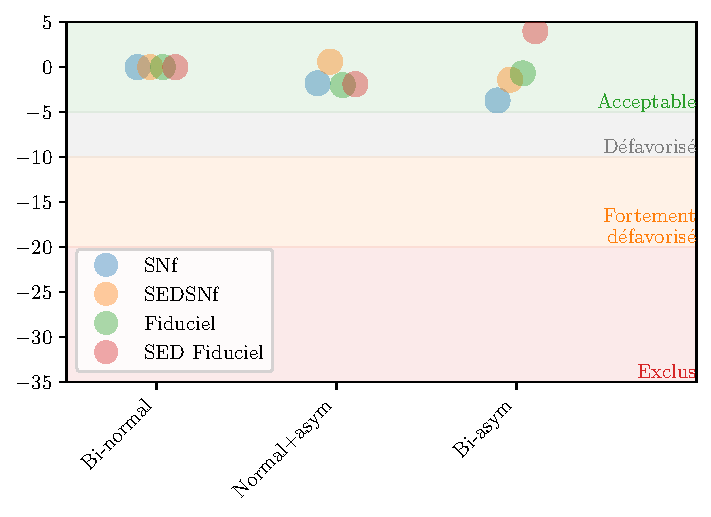
\includegraphics[width=.6\linewidth]{mass_comp_df-nobug}
    \caption[$\Delta$AIC entre le modèle Howell et les autres
    modèles]{$\Delta$AIC entre le modèle Howell et les autres modèles (voir
        Tableau~\ref{tab:modelcomp}). Tous les modèles sont dérivants. Les
        marqueurs bleus, orange, verts, rouges montrent les résultats lorsque
        l'analyse est effectuée sur l'échantillon SNF, SEDSNF, fiduciel,
        fiduciel avec SEDSNf, respectivement (voir légende). Les bandes de
        couleur illustrent la validité des modèles, d'acceptable ($\Delta$AIC >
        -5) à exclu ($\Delta$AIC < -20). En suivant ces valeurs d'AIC, tous les
        modèles sont compatibles entre eux.}
    \label{fig:mod_comp}
\end{figure}

\begin{figure}[htbp]
    \vspace*{-3cm}
    \centerfloat
    \includegraphics[width=1.1\linewidth]{mass_model_all_evol.pdf}
    \caption[Modèles implémentés et testés dans l'étude de l'évolution de
    l'étirement avec le redshift]{\scriptsize Modèles implémentés et testés dans
        l'étude de l'évolution de la masse avec le redshift. Les modèles Howell,
        Howell+asym et Howell asym sont tracés dans la colonne de gauche, du
        milieu et de droite, respectivement. Les échantillons sur lesquels ils
        sont ajustés correspondent aux lignes et à la couleur de fond du
        graphique~: SNf (bleu), SEDSNf (orange), fiduciel (vert), fiduciel avec
        SEDSNF (rouge)~; ce sont les mêmes couleurs que dans la
        Figure~\ref{fig:mod_comp}. Les quantités $\Delta(-2\ln(L))$ et
        $\Delta$AIC par rapport au modèle Howell de chaque ligne sont indiqués
        pour chaque modèle figure. Nous avons tracé dix réalisations des modèles
        selon la valeur du redshift moyen considéré, de la valeur la plus basse
        de notre échantillon ($z = 0,02$) à la valeur maximale des données
        totales (sans coupe en redshift) de SNLS ($z = 1,06$) représentés en
        couleur allant du jaune (bas redshift, plus vieil environnement) au
        violet (haut redshift, environnement jeune) et les distributions des
        populations jeune et vieille constituant le modèle total sont en gris
        pointillé et fin pointillé, respectivement. Nous y retrouvons
        l'information que tous les modèles sont compatibles en tant que bonnes
    représentations des données par rapport au modèle de base.}
    \label{fig:mod_all}
\end{figure}

\subsection{Sélection des modèles}\label{ssec:mmodsel}

Avec la multitude de modèles possibles pour établir nos \hostlib, nous avons dû
effectuer une sélection. Étant donné que notre but est d'associer de manière
cohérente un âge de SN définie par un redshift et une masse de galaxie hôte, une
caractéristique primordiale au modèle choisi est d'avoir une évolution de la
fraction de jeunes SNe~Ia physiquement cohérente avec les observations~; nous
nous attendons notamment à ce que la fraction de jeunes étoiles soit $\approx$ 1
pour les $M_* \gtrsim 10^7\si{\Msun}$, diminue progressivement jusqu'à $\approx
50\%$ pour $M_* \approx 10^{10}\si{\Msun}$ et continue sa progression vers 0
pour $M_* > 10^{10}\si{\Msun}$~; en effet, la position de la marche de magnitude
basée sur la masse est à $M_* = 10^{10}\si{\Msun}$ et cette limite constitue un
bon indicateur de l'âge d'une SN~Ia d'après~\cite{briday2022}.

Nous avons étudié cette évolution pour les différents modèles implémentés, dont
les résultats sont présentés Figure~\ref{fig:ypc}.

\begin{figure}[ht]
    \centerfloat
    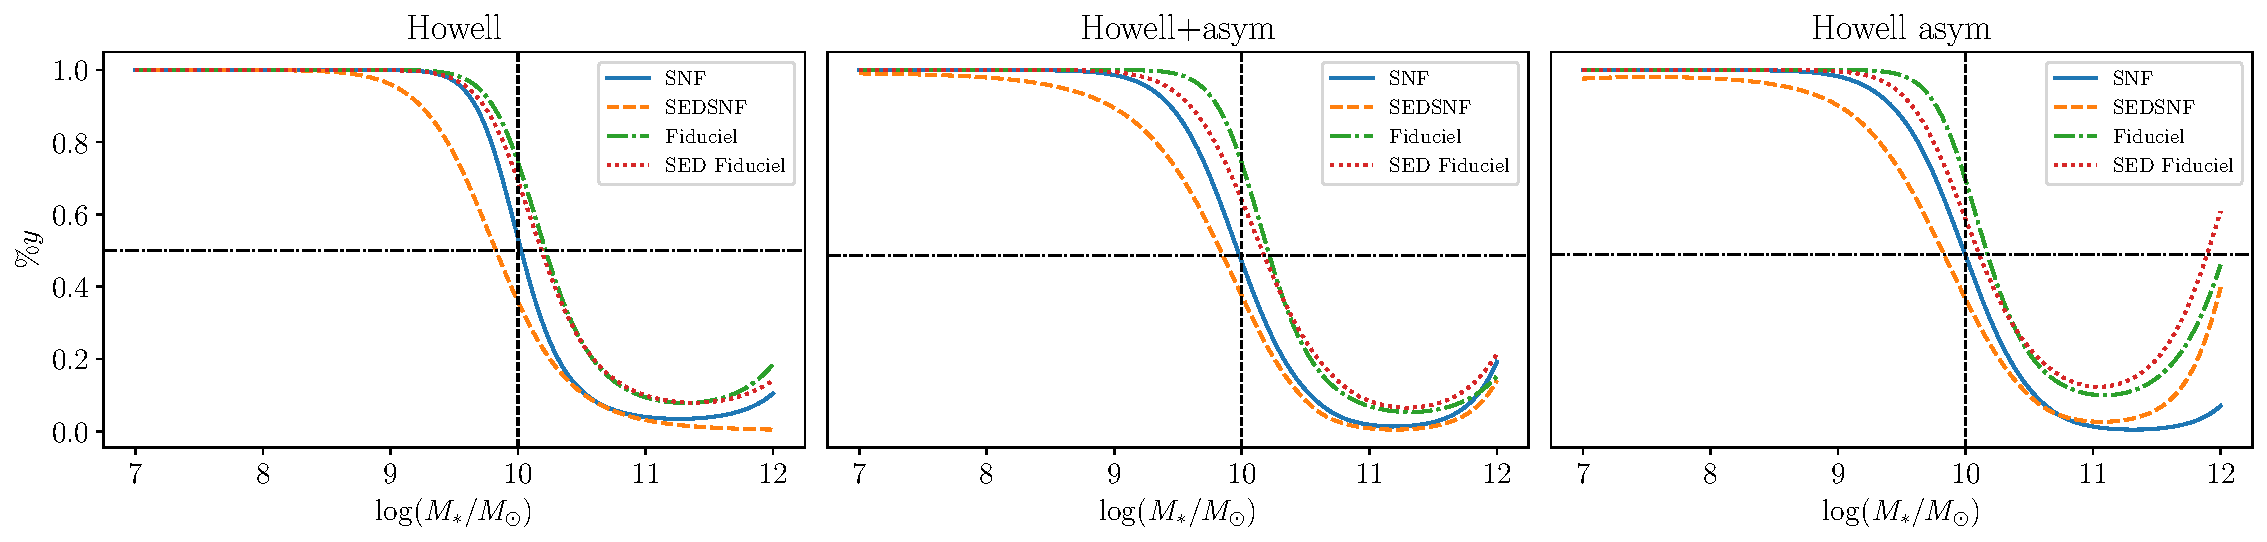
\includegraphics[width=1.2\linewidth]{model_mass_yfrac-best}
    \caption[Comparaison de la prédiction de l'évolution de la fraction de
    jeunes SNe~Ia en fonction de la masse de la galaxie hôte]{Comparaison de la
        prédiction de l'évolution de la fraction de jeunes SNe~Ia ($\%y$) en
        fonction de la masse de la galaxie hôte ($M_*$) pour chaque modèle et
        selon chaque échantillon utilisé pour l'ajustement. Alors que le sens de
        variation devrait être constant, pratiquement tous les modèles finissent
        par remonter après $M_* \approx 10^{11}\si{\Msun}$, sauf le modèle
        Howell ajusté sur SEDSNf. Nous excluons les modèles Howell+asym et
    Howell asym par ce critère.}
    \label{fig:ypc}
\end{figure}

Nous trouvons alors que tous les modèles finissent par présenter une remontée de
la fraction de jeunes étoiles quand la masse $M_* > 10^{11}\si{\Msun}$, sauf le
modèle Howell ajusté sur l'échantillon SEDSNf. Cela provient de l'incertitude
des courbes Gaussiennes des sous-populations jeunes étant bien plus larges que
celles des sous-populations vieilles, donnant pour les masses élevée un rapport
de probabilité en faveur des jeunes SNe~Ia. Ceci ne correspondant pas à une
réalité physique, nous rejetons tous les modèles Howell+asym et Howell asym de
notre étude à partir de ces résultats.

Parmi les modèles Howell, seul celui ajusté sur SNf passe en effet par 50\% à
$M_*=10^{10}\si{\Msun}$. Nous conservons ainsi les modèles Howell ajusté sur
SEDSNf et le modèle Howell ajusté sur SNf. Les valeurs des paramètres les
décrivant sont indiquées Tableau~\ref{tab:modelresults}.

\begin{table}[ht]
    \centerfloat
    \caption[Valeurs des paramètres issus des meilleurs ajustement du modèle
    Howell sur les échantillons SNF et SEDSNf]{Valeurs des paramètres issus des
    meilleurs ajustement du modèle Howell sur les échantillons SNF et SEDSNf.}
    \label{tab:modelresults}
    \begin{tabular}{lcccc}
        \toprule
        Échantillon              &
                $\mu_{\rm y} $   &
                $\sigma_{\rm y}$ &
                $\mu_{\rm o} $   &
                $\sigma_{\rm o}$ \\
        \midrule
        SNf    & $9.36  \pm 0.06$
               & $0.64  \pm 0.04$
               & $10.58 \pm 0.04$
               & $0.38  \pm 0.04$
               \\
        SEDSNf & $9.32  \pm 0.07$
               & $0.58  \pm 0.05$
               & $10.34 \pm 0.07$
               & $0.51  \pm 0.06$
               \\
        \bottomrule
    \end{tabular}
\end{table}

\subsection{Génération des \hostlib}\label{ssec:inpgen}

Avec les modélisations de la masse et de l'étirement en fonction du redshift,
nous pouvons à présent lire les entrées des \hostlib\ BP, et à partir d'un
redshift générer une liste de masses et d'étirements. Cela nous permettra
ensuite de faire correspondre la masse de la \hostlib\ avec celles de la liste
générée, et d'attribuer une valeur d'étirement qui remplacera celle
de~\citetalias{popovic2021a}.

Cette étape est réalisée avec le module Python
\texttt{SNprop}\footnote{\label{fn:snprop}\href{
    https://github.com/MickaelRigault/snprop}
{https://github.com/MickaelRigault/snprop}}. Ce processus prend la fraction
attendue de jeunes étoiles en utilisant $\delta(z)$ donnée
Équation~\ref{eq:deltaz}. Il assigne une qualité «~jeune~» (LsSFR = 1) ou
«~vieille~» (LsSFR = 0) au tirage qui va suivre en prenant un nombre aléatoire
$r$ entre 0 et 1 et en le comparant à la valeur de la fraction susmentionnée. Si
$r < \delta(z)$, alors la SN simulée sera jeune et inversement. Plus $z$
augmente et plus $\delta(z)$ augmente, et donc plus la probabilité d'être
assigné jeune augmente. Ceci est présenté Figure~\ref{fig:deltaz}.

\begin{figure}[]
    \centering
    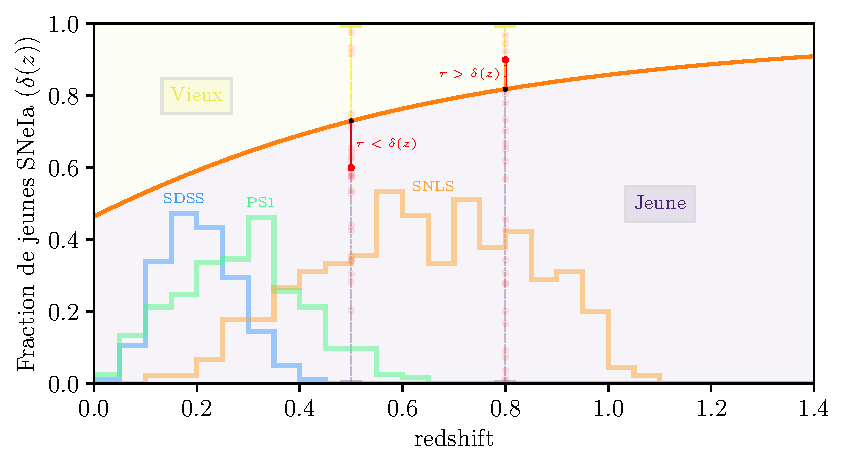
\includegraphics[width=\linewidth]{deltaz_hist_yo-random.pdf}
    \caption[Représentation du choix de l'âge d'une SN et de l'assignation de
    masse et d'étirement en fonction du redshift]{Représentation du choix de
        l'âge d'une SN et de l'assignation de masse et d'étirement en fonction
        du redshift du module Python \texttt{SNprop}\footnoteref{fn:snprop}.
        \textit{Orange}~: fraction estimée de jeunes SNe~Ia en fonction du
        redshift. \textit{Histogrammes}~: nombres de SNe~Ia des 3 sondages
        principaux de l'échantillon Pantheon \citep{scolnic2018} (pas à
        l'échelle). \textit{Lignes rouges verticales}~: pour chaque $z$ de la
        \hostlib, un nombre aléatoire $r$ entre 0 et 1 est tiré~: s'il est
        supérieur (inférieur) à $\delta(z)$ à ce redshift, alors la SN sera
        assignée vieille (jeune) et les valeurs de masse et d'étirement générées
        seront tirées des distributions sous-jacentes vieilles (jeunes) des
    paramètres correspondants.}
    \label{fig:deltaz}
\end{figure}

Cette étape est réalisée \num{1000} fois pour chaque redshift de la \hostlib,
donnant une table de redshift, LsSFR (0 ou 1), masse et étirement de \num{1000}
entrées, puis une correspondance est effectuée entre toutes les masses tirées et
la masse de la \hostlib\ pour trouver celle qui en est la plus proche. Nous
prenons alors la valeur d'étirement associée et remplaçons celle de la \hostlib.
Au même moment, nous entrons la valeur de l'âge (0 ou 1) dans une nouvelle
colonne \texttt{LOGsSFR}~; ceci conclut la confection des \hostlib\ NN. Les
\hostlib\ NR possèdent un autre colonne supplémentaire, où à chaque valeur de
\texttt{LOGsSFR} est associée une valeur de \texttt{SNMAGSHIFT}, de +0,065 pour
\texttt{LOGsSFR} = 1 (jeune, moins lumineuse) et de -0,065 pour \texttt{LOGsSFR}
= 0 (vieille, plus lumineuse), qui remplacent le valeurs de marche de magnitude
basées sur la masse implémentées dans les autres approches et qui sont associées
au \wgtmap.

Selon le modèle de masse utilisé, il y a donc différentes \hostlib, qui
correspondent à nos simulations. Nous recensons donc~:
\begin{enumerate}
    \item Les \hostlib\ avec le modèle Howell ajusté sur SEDSNf~;
    \item Les \hostlib\ avec le modèle Howell ajusté sur SNf~;
\end{enumerate}
et pour reproduire artificiellement la descente de la fraction de jeunes étoiles
en fonction de la masse attendue, nous avons également~:
\begin{enumerate}[resume]
    \item Les \hostlib\ avec le modèle Howell ajusté sur SNf, mais pour
        lesquelles les entrées de $M_* > 10^{11}\si{\Msun}$ sont automatiquement
        associées à des SNe~Ia âgées~; cette simulation est appelée «~SNfsupp~»
        pour «~suppressed~» («~réprimé~»).
\end{enumerate}

\section{Implémentation}\label{sec:snaimpl} 

Nous traitons maintenant de l'implémentation de ces simulations. Dans un premier
lieu nous introduisons les types de simulations (Section~\ref{ssec:type}) et la
nomenclature utilisée (Section~\ref{ssec:nom}), puis la manière de contrôler le
nombre de SNe~Ia simulées et notre choix de réalisation
(Section~\ref{ssec:ngen}), avant de présenter la méthode de comparaison de
correspondance entre les données réelles et les données simulées
(Section~\ref{ssec:comp}).

\subsection{Types de simulations}\label{ssec:type}

Nous pouvons implémenter différentes manières d'effectuer ces simulations, que
nous appelons «~types~».

Idéalement, notre approche serait de simuler 100 fois des échantillons de la
taille de l'échantillon de Pantheon ($\approx \num{1000}$) et de combiner les
résultats, permettant ainsi d'avoir des incertitudes statistiques réalistes~; un
tel type de simulation était appelé «~SSIZE~» pour «~sample sized~» (de la
taille des échantillons), et prend un temps de calcul considérable.

Le plus simple et moins coûteux en temps a été de simuler un échantillon d'une
taille conséquente ($\approx \num{13 000}$) une fois pour chaque simulation avec
un BiasCor 50 fois plus grand, type de simulation appelé «~FULL~» (complet).

Des tentatives de simulation avec des données simulées en très grand nombre ont
été implémentées, nommées «~VFULL~» pour «~very full~» (très complet).

D'autres types ont été implémentés, mais la complexité des simulations avec
\snana\ nous a forcæ à modifier les paramètres de simulation jusqu'au dernier
moment, rendant impossible le fait d'effectivement réaliser ces types de
simulations, et nous ne présentons ici que les résultats «~FULL~».

\subsection{Nomenclature des simulations}\label{ssec:nom}

Par chacun des modèles utilisés et donc chacune des simulations, nous générons
les échantillons LOWZ, SDSS, PS1 et SNLS avec les \hostlib\ SK, BP, NN et NR
(que nous appelons les «~saveurs~» de simulation), afin de comparer les
résultats finaux de ces simulations avec les données de Pantheon et voir
l'impact de ces différentes corrélations à l'environnement sur la cosmologie. À
chaque échantillon simulé est associé un échantillon BiasCor qui sera combiné
sur les différents sondages pour chaque saveur. Tous ces échantillons simulés
sont conservés pour pouvoir utiliser les données d'une saveur et de les corriger
avec le BiasCor d'une autre saveur~: l'idée derrière cette pratique est de
générer des données avec certaines hypothèses et de les ajuster en en utilisant
d'autres pour connaître le potentiel biais dû au fait de méconnaître la physique
réelle qui régit les propriétés intrinsèques des SNe~Ia.

Ainsi, la nomenclature de nos simulations suit la logique suivante~:
\begin{center}
    \begin{tikzpicture}[]
        \node[anchor=center] (name) at (0,0)
            {\textcolor{Orchid}{FULL}\_\textcolor{cornflowerblue}{SEDSNF}\_\textcolor{limegreen}{SK}\_\textcolor{orange}{NR}};
        \node[inner sep=0] (typeb) at ([shift={(0,3pt)}]name.south west) {};
        \node[] (leftb) at ([shift={(20pt,3pt)}]name.south west) {};
        \node[inner sep=0] (simub) at ([shift={(48pt,0)}]leftb.center) {};
        \node[inner sep=0] (flabb) at ([shift={(39pt,0)}]simub.center) {};
        \node[inner sep=0] (flasb) at ([shift={(0,3pt)}]name.south east) {};
        \node[below left =of typeb, color=Orchid] (type)
            {Type};
        \node[below left =of simub, color=cornflowerblue, anchor=north] (simu)
            {Simulation/modèle};
        \node[below right=of flabb, color=limegreen, anchor=north] (flab)
            {Données};
        \node[below right=of flasb, color=orange] (flas)
            {BiasCor};
        \draw[-stealth] (type) -- (typeb);
        \draw[-stealth] (simu) -- (simub);
        \draw[-stealth] (flab) -- (flabb);
        \draw[-stealth] (flas) -- (flasb);
    \end{tikzpicture}
\end{center}

\subsection{Contrôle du nombre de SNe~Ia simulées~:\texttt{NGEN}}\label{ssec:ngen}

Pour comparer de manière cohérente les données simulées aux données réelles, il
faut que le ratio des données de chaque sondage de l'échantillon simulé
corresponde au ratio des données de chaque sondage de l'échantillon réel. Ceci
s'effectue \textit{via} un paramètre appelé \texttt{NGEN}, décrivant le nombre
d'années de sondage simulé. Il permet de contrôler plus ou moins précisément le
nombre de SNe~Ia simulées, puisque chaque sondage a sa propre efficacité
spectroscopique qui, à chaque simulation, opère une sélection des données
conservées (voir Chapitre~\ref{ch:snana}). Notamment, puisque l'efficacité
spectroscopique de l'échantillon LOWZ est particulièrement faible, il nécessite
un grand \texttt{NGEN} dans nos fichiers de configurations. De plus, la
correction par \bbc\ réduit l'échantillon en ne conservant que les données qui
possèdent une correction~; ainsi, en plus de l'ajustement avec \texttt{NGEN},
nous avons implémenté une sélection aléatoire des données de chaque sondage pour
reproduire les ratio attendus. Nous indiquons dans le Tableau~\ref{tab:ratio} le
nombre de données pour les données réelles et pour nos simulations à chaque
stage de sélection.

% \begin{table}
%     \centering
%     \caption{Number of data in Pantheon and relative ratio with respect to the
%     smallest sample, LOWZ}
%     \label{tab:ratio}
%     \begin{tabular}{lcc}
%         \toprule
%         Survey & Number & Ratio/LOWZ \\
%         \midrule
%         LOWZ   & 172    & 1.00 \\
%         SDSS   & 335    & 1.95 \\
%         PS1    & 279    & 1.62 \\
%         SNLS   & 236    & 1.37 \\
%         \bottomrule
%     \end{tabular}
% \end{table}

\begin{table}
    \centerfloat
    \caption[Nombre de données de nos différentes simulations]{Nombre de
        données avant, après l'ajustement par \bbc, et après
        l'échantillonnage nécessaire à la reproduction des ratio
    observés dans l'échantillon Pantheon \citep{scolnic2018}.}
    \label{tab:ratio}
    \begin{adjustbox}{max width=\textwidth}
        \begin{threeparttable}
            % \begin{tabular}{cllcccc|cccc|cccccc}
            \begin{tabular}{cllcccccccccccccc}
                \toprule & & &
                \multicolumn{4}{c}{Avant \bbc} &
                \multicolumn{4}{c}{Après \bbc} &
                \multicolumn{4}{c}{Échantillonné} &
                \multirow{2}[1]{*}{Total\tnote{1}} &
                \multirow{2}[1]{*}{BiasCor\tnote{2}}
                \\
                \cmidrule(lr){4-7} \cmidrule(lr){8-11} \cmidrule(lr){12-15}
                Simulation & \multicolumn{2}{c}{Saveurs} &
                LOWZ       & SDSS    & PS1 & SNLS &
                LOWZ       & SDSS    & PS1 & SNLS &
                LOWZ       & SDSS    & PS1 & SNLS & &
                \\
                \midrule
                Pantheon &     &     &
                         &     &     &     &
                172      & 335 & 279 & 236 &
                         &     &     &     &
                1022     & \\
                \midrule
                \multirow{16}[6]{*}{SNFSUPP} & \multirow{4}{*}{SK} & SK &
                3110                         & 3306   & 6768 & 5340 &
                2346                         & 2443   & 5477 & 3067 &
                2346                         & 2443   & 5477 & 3067 &
                13333                        & \multirow{4}[0]{*}{932916}
                \\
                      &      & BP   &
                3110  & 3306 & 6768 & 5340 &
                2290  & 2344 & 5368 & 2845 &
                2290  & 2344 & 5368 & 2845 &
                12847 &
                \\
                      &      & NN   &
                3110  & 3306 & 6768 & 5340 &
                2242  & 2348 & 5413 & 2895 &
                2242  & 2348 & 5413 & 2895 &
                12898 &
                \\
                      &      & NR   &
                3110  & 3306 & 6768 & 5340 &
                2242  & 2348 & 5413 & 2895 &
                2242  & 2348 & 5413 & 2895 &
                12898 &
                \\ \cmidrule(lr){2-17}
                       & \multirow{4}{*}{BP}     & SK   &
                2594   & 3199                    & 6557 & 5274 &
                1806   & 2248                    & 5050 & 3212 &
                1806   & 2248                    & 5050 & 3212 &
                12316  & \multirow{4}{*}{880488}
                \\
                      &      & BP   &
                2594  & 3199 & 6557 & 5274 &
                1821  & 2268 & 5206 & 3167 &
                1821  & 2268 & 5206 & 3167 &
                12462 &
                \\
                      &      & NN   &
                2594  & 3199 & 6557 & 5274 &
                1724  & 2263 & 5213 & 3197 &
                1724  & 2263 & 5213 & 3197 &
                12397 &
                \\
                      &      & NR   &
                2594  & 3199 & 6557 & 5274 &
                1724  & 2263 & 5213 & 3197 &
                1724  & 2263 & 5213 & 3197 &
                12397 &
                \\ \cmidrule(lr){2-17}
                      & \multirow{4}{*}{NN}     & SK   &
                3008  & 3188                    & 6634 & 5280 &
                2166  & 2191                    & 4986 & 3096 &
                2166  & 2191                    & 4986 & 3096 &
                12439 & \multirow{4}{*}{902775}
                \\
                      &      & BP   &
                3008  & 3188 & 6634 & 5280 &
                2152  & 2201 & 5115 & 3010 &
                2152  & 2201 & 5115 & 3010 &
                12478 &
                \\
                      &      & NN   &
                3008  & 3188 & 6634 & 5280 &
                2252  & 2215 & 5226 & 3094 &
                2252  & 2215 & 5226 & 3094 &
                12787 &
                \\
                      &      & NR   &
                3008  & 3188 & 6634 & 5280 &
                2252  & 2215 & 5226 & 3094 &
                2252  & 2215 & 5226 & 3094 &
                12787 &
                \\ \cmidrule(lr){2-17}
                      & \multirow{4}{*}{NR}     & SK   &
                3106  & 3200                    & 6616 & 5183 &
                2237  & 2210                    & 4992 & 3022 &
                2237  & 2210                    & 4992 & 3022 &
                12461 & \multirow{4}{*}{902775}
                \\
                      &      & BP   &
                3106  & 3200 & 6616 & 5183 &
                2216  & 2219 & 5111 & 2929 &
                2216  & 2219 & 5111 & 2929 &
                12475 &
                \\
                      &      & NN   &
                3106  & 3200 & 6616 & 5183 &
                2321  & 2243 & 5223 & 3011 &
                2321  & 2243 & 5223 & 3011 &
                12798 &
                \\
                      &      & NR   &
                3106  & 3200 & 6616 & 5183 &
                2321  & 2243 & 5223 & 3011 &
                2321  & 2243 & 5223 & 3011 &
                12798 &
                \\
                \midrule\midrule
                \multirow{16}[6]{*}{SNF} & \multirow{4}{*}{SK} & SK   &
                3110                     & 3306                & 6768 & 5340 &
                2346                     & 2443                & 5477 & 3067 &
                2346                     & 2443                & 5477 & 3067 &
                13333                    & \multirow{4}{*}{932916}
                \\
                       &      & BP   &
                3110   & 3306 & 6768 & 5340 &
                2290   & 2344 & 5368 & 2845 &
                2290   & 2344 & 5368 & 2845 &
                12847  &
                \\
                       &      & NN   &
                3110   & 3306 & 6768 & 5340 &
                2242   & 2353 & 5456 & 2886 &
                2242   & 2353 & 5456 & 2886 &
                12937  &
                \\
                       &      & NR   &
                3110   & 3306 & 6768 & 5340 &
                2242   & 2353 & 5456 & 2886 &
                2242   & 2353 & 5456 & 2886 &
                12937  &
                \\ \cmidrule(lr){2-17}
                       & \multirow{4}{*}{BP}     & SK   &
                2594   & 3199                    & 6557 & 5274 &
                1806   & 2248                    & 5050 & 3212 &
                1806   & 2248                    & 5050 & 3212 &
                12316  & \multirow{4}{*}{880488}
                \\
                       &      & BP   &
                2594   & 3199 & 6557 & 5274 &
                1821   & 2268 & 5206 & 3167 &
                1821   & 2268 & 5206 & 3167 &
                12462  &
                \\
                       &      & NN   &
                2594   & 3199 & 6557 & 5274 &
                1718   & 2263 & 5229 & 3210 &
                1718   & 2263 & 5229 & 3210 &
                12420  &
                \\
                       &      & NR   &
                2594   & 3199 & 6557 & 5274 &
                1718   & 2263 & 5229 & 3210 &
                1718   & 2263 & 5229 & 3210 &
                12420  &
                \\ \cmidrule(lr){2-17}
                       & \multirow{4}{*}{NN}     & SK   &
                3037   & 3205                    & 6644 & 5305 &
                2180   & 2235                    & 5117 & 3131 &
                2180   & 2235                    & 5117 & 3131 &
                12663  & \multirow{4}{*}{907904}
                \\
                       &      & BP   &
                3037   & 3205 & 6644 & 5305 &
                2165   & 2236 & 5176 & 3051 &
                2165   & 2236 & 5176 & 3051 &
                12628  &
                \\
                       &      & NN   &
                3037   & 3205 & 6644 & 5305 &
                2264   & 2250 & 5288 & 3113 &
                2264   & 2250 & 5288 & 3113 &
                12915  &
                \\
                       &      & NR   &
                3037   & 3205 & 6644 & 5305 &
                2264   & 2250 & 5288 & 3113 &
                2264   & 2250 & 5288 & 3113 &
                12915  &
                \\ \cmidrule(lr){2-17}
                       & \multirow{4}{*}{NR}     & SK   &
                3097   & 3204                    & 6607 & 5193 &
                2239   & 2224                    & 5068 & 3054 &
                2239   & 2224                    & 5068 & 3054 &
                12585  & \multirow{4}{*}{907904}
                \\
                       &      & BP   &
                3097   & 3204 & 6607 & 5193 &
                2221   & 2228 & 5136 & 2968 &
                2221   & 2228 & 5136 & 2968 &
                12553  &
                \\
                       &      & NN   &
                3097   & 3204 & 6607 & 5193 &
                2326   & 2246 & 5249 & 3038 &
                2326   & 2246 & 5249 & 3038 &
                12859  &
                \\
                       &      & NR   &
                3097   & 3204 & 6607 & 5193 &
                2326   & 2246 & 5249 & 3038 &
                2326   & 2246 & 5249 & 3038 &
                12859  &
                \\
                \midrule\midrule
                \multirow{16}[6]{*}{SEDSNF} & \multirow{4}{*}{SK}  & SK &
                3110                        & 3306   & 6768 & 5340 &
                2346                        & 2443   & 5477 & 3067 &
                2346                        & 2443   & 5477 & 3067 &
                13333                       & \multirow{4}{*}{932916}
                \\
                       &      & BP   &
                3110   & 3306 & 6768 & 5340 &
                2290   & 2344 & 5368 & 2845 &
                2290   & 2344 & 5368 & 2845 &
                12847  &
                \\
                       &      & NN   &
                3110   & 3306 & 6768 & 5340 &
                2241   & 2372 & 5460 & 2928 &
                2241   & 2372 & 5460 & 2928 &
                13001  &
                \\
                       &      & NR   &
                3110   & 3306 & 6768 & 5340 &
                2241   & 2372 & 5460 & 2928 &
                2241   & 2372 & 5460 & 2928 &
                13001  &
                \\ \cmidrule(lr){2-17}
                       & \multirow{4}{*}{BP}     & SK   &
                2594   & 3199                    & 6557 & 5274 &
                1806   & 2248                    & 5050 & 3212 &
                1806   & 2248                    & 5050 & 3212 &
                12316  & \multirow{4}{*}{880488}
                \\
                       &      & BP   &
                2594   & 3199 & 6557 & 5274 &
                1821   & 2268 & 5206 & 3167 &
                1821   & 2268 & 5206 & 3167 &
                12462  &
                \\
                       &      & NN   &
                2594   & 3199 & 6557 & 5274 &
                1744   & 2291 & 5223 & 3216 &
                1744   & 2291 & 5223 & 3216 &
                12474  &
                \\
                       &      & NR   &
                2594   & 3199 & 6557 & 5274 &
                1744   & 2291 & 5223 & 3216 &
                1744   & 2291 & 5223 & 3216 &
                12474  &
                \\ \cmidrule(lr){2-17}
                       & \multirow{4}{*}{NN}     & SK   &
                2965   & 3192                    & 6642 & 5310 &
                2184   & 2180                    & 4982 & 3141 &
                2184   & 2180                    & 4982 & 3141 &
                12487  & \multirow{4}{*}{904605}
                \\
                       &      & BP   &
                2965   & 3192 & 6642 & 5310 &
                2149   & 2169 & 5093 & 3067 &
                2149   & 2169 & 5093 & 3067 &
                12478  &
                \\
                       &      & NN   &
                2965   & 3192 & 6642 & 5310 &
                2250   & 2242 & 5250 & 3142 &
                2250   & 2242 & 5250 & 3142 &
                12884  &
                \\
                       &      & NR   &
                2965   & 3192 & 6642 & 5310 &
                2250   & 2242 & 5250 & 3142 &
                2250   & 2242 & 5250 & 3142 &
                12884  &
                \\ \cmidrule(lr){2-17}
                       & \multirow{4}{*}{NR}     & SK   &
                3067   & 3193                    & 6583 & 5223 &
                2253   & 2170                    & 4925 & 3063 &
                2253   & 2170                    & 4925 & 3063 &
                12411  & \multirow{4}{*}{904605}
                \\
                       &      & BP   &
                3067   & 3193 & 6583 & 5223 &
                2219   & 2152 & 5034 & 3005 &
                2219   & 2152 & 5034 & 3005 &
                12410  &
                \\
                       &      & NN   &
                3067   & 3193 & 6583 & 5223 &
                2323   & 2227 & 5194 & 3075 &
                2323   & 2227 & 5194 & 3075 &
                12819  &
                \\
                       &      & NR   &
                3067   & 3193 & 6583 & 5223 &
                2323   & 2227 & 5194 & 3075 &
                2323   & 2227 & 5194 & 3075 &
                12819  &
                \\
                \bottomrule
            \end{tabular}
            \begin{tablenotes}[flushleft]
                \item [1] \small Les modèles étant spécifiques aux \hostlib\ NN
                    et NR, le nombre de données des simulations ne faisant
                    intervenir que BP et SK sont les mêmes pour les 3 modèles.
                \item [2] \small Les échantillons BiasCor indiqués sont ceux de
                    la saveur utilisée pour les données.
            \end{tablenotes}
        \end{threeparttable}
    \end{adjustbox}
\end{table}

\begin{itemize}
    \item Plot HOSTLIBs parameters?
    \item Weigthmaps, plot them?
    \item Talk about NGENs and how they are made to fit to the ratio in
        Pantheon?
\end{itemize}

\subsection{Comparaison des données simulées aux données réelles}\label{ssec:comp}

Avant de comparer les résultats cosmologiques, nous nous sommes intéressæ à la
correspondance entre les données simulées et les données réelles afin
d'apprécier les changements sur les distributions des différentes saveurs de
simulation. Nous étudions pour cela les distributions d'étirement en fonction du
redshift et les distributions d'étirement en fonction de la masse de la galaxie
hôte. Nous les représentons en histogrammes 2D en couleurs pour les données
simulées, et en points dispersés pour les données réelles. Pour déterminer
l'accord entre ces deux échantillons de manière quantitative, nous avons
utilisé une estimation par noyau pour convertir les données simulées en densité
de probabilité bi-dimensionnelle, permettant de calculer un $\chi^2$ entre les
données réelles et le noyau. Un exemple est donné Figure~\ref{fig:2dhex}.

% Before comparing the $w$ v $\Omega_m$ values, we looked at the correspondence
% between simulated data and actual data to ensure the improvement of our
% LsSFR-based approach. The main idea being the evolution of the underlying
% stretch distribution as a function of redshift, we represented $x_1$ v $z$ in
% log-scale using a 2D hexagonal colored histogram for the simulated data and dots
% for the Pantheon values. We also looked at the $x_1$ v $M\mathrm{host}$ plot to
% ponder the relationship these two main characteristics of the SNe~Ia on one hand
% and the host galaxies on the other (see \ref{fig:P21vN21}). We then computed a
% 2D kernel of each set of parameters based on the simulations and determined the
% associated $\chi^2$ between the data and the kernels. The results are summarized
% in Table \ref{tab:chi2comp} and the code in the \textit{SNprop} module.

\begin{figure*}
    \centering
    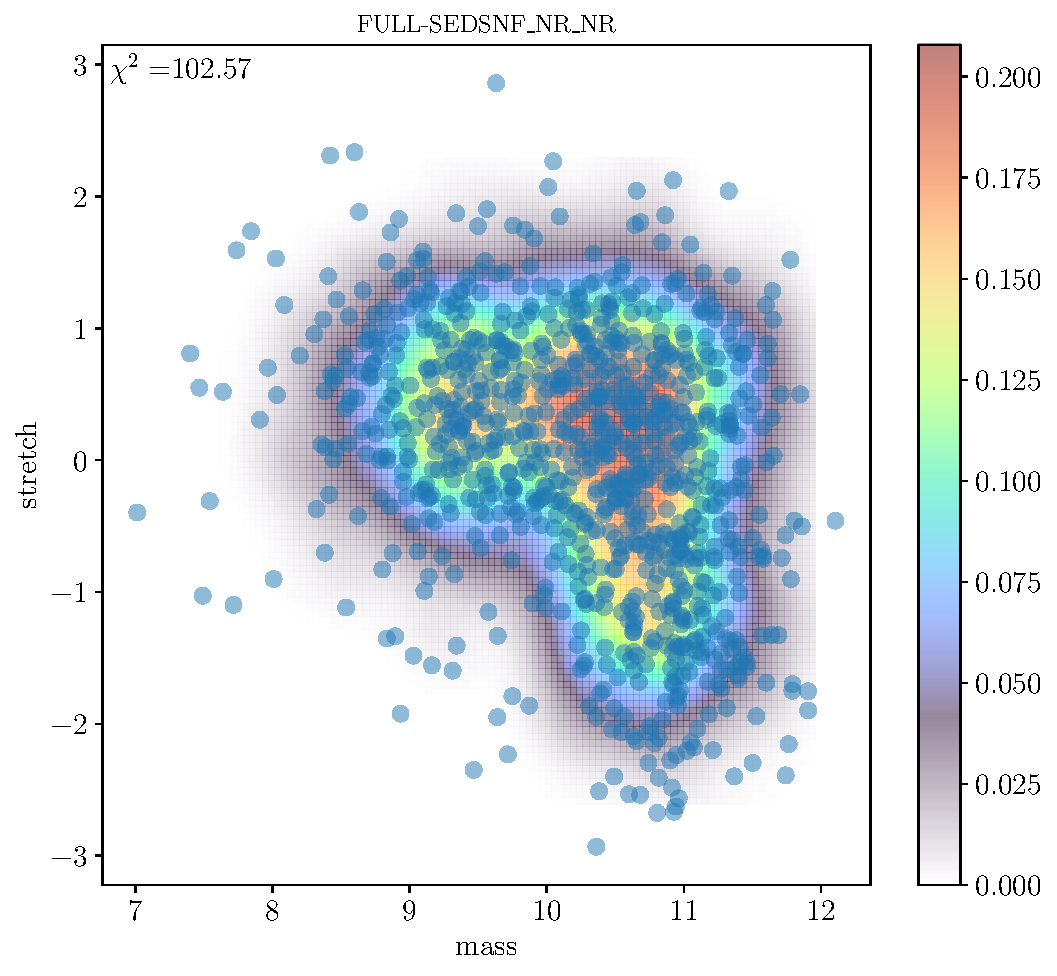
\includegraphics[width=.5\linewidth]{FULL-SEDSNF_NR_NR_MS_kernel}
    \caption[Accord entre les données réelles et simulées avec le modèle SEDSNf
    pour les saveurs NR\_NR]{Accord entre les données réelles et simulées avec
    le modèle SEDSNf pour les saveurs NR\_NR}
    \label{fig:2dhex}
\end{figure*}

\begin{table}
    \centering
    \caption{Comparison of the relative ability of each HOSTLIB implementation
    to describe the data. For each HOSTLIB a 2D KDE is computed from the simulated
    data and used to determine said $\chi^2$.}
    \label{tab:chi2comp}
    \begin{tabular}{c|cc}
        \hline\hline
                & \multicolumn{2}{c}{$\chi^2$}
        \\
        HOSTLIB & $x_1$ v $z$ & $x_1$ v $M_\mathrm{host}$
        \\\hline
        P21     & ????        & ????
        \\
        N21     & ????        & ????
        \\
        \hline
    \end{tabular}
\end{table}

The numerical values follow what was already clear on the figures: it fits best.

\section{Résultats}\label{sec:simres}
What we want is not so much $w$ than $\Delta w$ wrt. best current work. We find
x\% and here are the contours.

\section{Discussion}\label{sec:simdisc}
We expected to have a higher/lower, and we got that.

\section{Conclusion}\label{sec:simccl}

Should be nice.


\clearpage

\thispagestyle{plain}
% \vspace*{-3cm}
\vfill
\minilof
\vfill
\minilot
\vfill

\bibliographystyle{../main/aa_url}
\shorthandoff{:}
\bibliography{../chapters/99_references}

\end{document}
